\section{Proposed Methodology}
\label{sec:proposed_method}

Nebium is architected as a modernized, decoder-only causal transformer \parencite{vaswani2017attention} optimized specifically for the structural and temporal dynamics of chess sequence modeling. Rather than adopting an unmodified vanilla GPT configuration with standard learned absolute position embeddings and Post-LayerNorm \parencite{deleo2022learning}, Nebium incorporates exisiting three state-of-the-art architectural methods such as \textbf{Rotary Position Embeddings (RoPE)} \parencite{su2024roformer}, \textbf{Swish-Gated Linear Units (SwiGLU)} \parencite{shazeer2020glu}, and \textbf{Root Mean Square Normalization (RMSNorm)} \parencite{zhang2019root}. The holistic pipeline is presented in following Figure~\ref{fig:architecture}.

\subsection{End-to-End Architectural Pipeline}
\label{sec:arch_pipeline}
Given an input token sequence of length $T$, $\mathbf{x}_{1:T} = (x_1, \dots, x_T) \in \mathbb{N}^T$, the sequence is first mapped into dense representations via a learned token embedding matrix $\mathbf{W}_e \in \mathbb{R}^{V \times d_{\text{model}}}$:
\begin{equation}
    \mathbf{h}_0 = \text{Dropout}\left(\mathbf{W}_e[\mathbf{x}_{1:T}], \, p_{\text{drop}}\right) \in \mathbb{R}^{T \times d_{\text{model}}}
\end{equation}
Then embeddings traverse a stack of $L = 6$ identical Transformer Blocks. Each block $\ell \in \{1, \dots, L\}$ applies a pre-normalized residual formulation:
\begin{align}
    \mathbf{u}_\ell &= \mathbf{h}_{\ell-1} + \text{MHSA}\left(\text{RMSNorm}(\mathbf{h}_{\ell-1})\right) \\
    \mathbf{h}_\ell &= \mathbf{u}_\ell + \text{SwiGLU}\left(\text{RMSNorm}(\mathbf{u}_\ell)\right)
\end{align}
The final representation $\mathbf{h}_L$ undergoes RMSNorm before linear projection to a next-token vocabulary logits via $\mathbf{W}_{\text{head}} \in \mathbb{R}^{d_{\text{model}} \times V}$:
\begin{equation}
    \mathbf{z}_t = \mathbf{W}_{\text{head}} \, \text{RMSNorm}(\mathbf{h}_{L, t}) \in \mathbb{R}^V
\end{equation}

Table~\ref{tab:model_hyperparams} lists the structural configurations and hyperparameter settings for Nebium.

\begin{table}[H]
\centering
\small
\caption{Architectural specifications and parameter configurations for Nebium.}
\label{tab:model_hyperparams}
\begin{tabularx}{\linewidth}{l l X}
\toprule
\textbf{Hyperparameter} & \textbf{Value / Dimension} & \textbf{Design Rationale and Technical Function} \\
\midrule
Vocabulary Size & $V = 5,000$ & Domain-trained BPE merges common coordinate sequences and opening pairs without vocabulary explosion \\
Embedding Dimension & $d_{\text{model}} = 512$ & Provides latent capacity for piece-square interactions while matching head dimension $d_k = 64$ \\
Number of Layers & $L = 6$ & Provides hierarchical depth for multi-ply tactical reasoning while maintaining stable gradient backpropagation \\
Attention Heads & $h = 8$ & Divides embeddings into 8 parallel projection subspaces ($d_k = d_{\text{model}}/h = 64$) aligned with tensor cores \\
FFN Expansion Dim & $d_{ff} = 1,368$ & Scaled to $\frac{2}{3} \times 4 d_{\text{model}}$ (rounded to multiple of 8) to match the parameter count of conventional FFNs \\
Positional Encoding & Rotary (RoPE) & Encodes relative ply offsets directly into query-key inner products, supporting sequence length extrapolation \\
Activation Function & SwiGLU & Bilinear gating improves non-linear expressiveness and gradient propagation relative to GELU \\
Layer Normalization & RMSNorm & Normalizes feature scale without mean-centering, cutting normalization latency and stabilizing FP16 training \\
Dropout Rate & $p_{\text{drop}} = 0.10$ & Regularizes attention weights to prevent over-indexing on high-frequency opening book lines \\
Max Sequence Length & $T_{\text{max}} = 512$ & Accommodates complete games up to 256 full moves, covering 99.1\% of competitive matches \\
Total Parameters & 28.4 Million & Compact footprint enabling sub-10~ms CPU generation within 128~MB of system RAM \\
\bottomrule
\end{tabularx}
\end{table}

\begin{figure}[H]
  \centering
  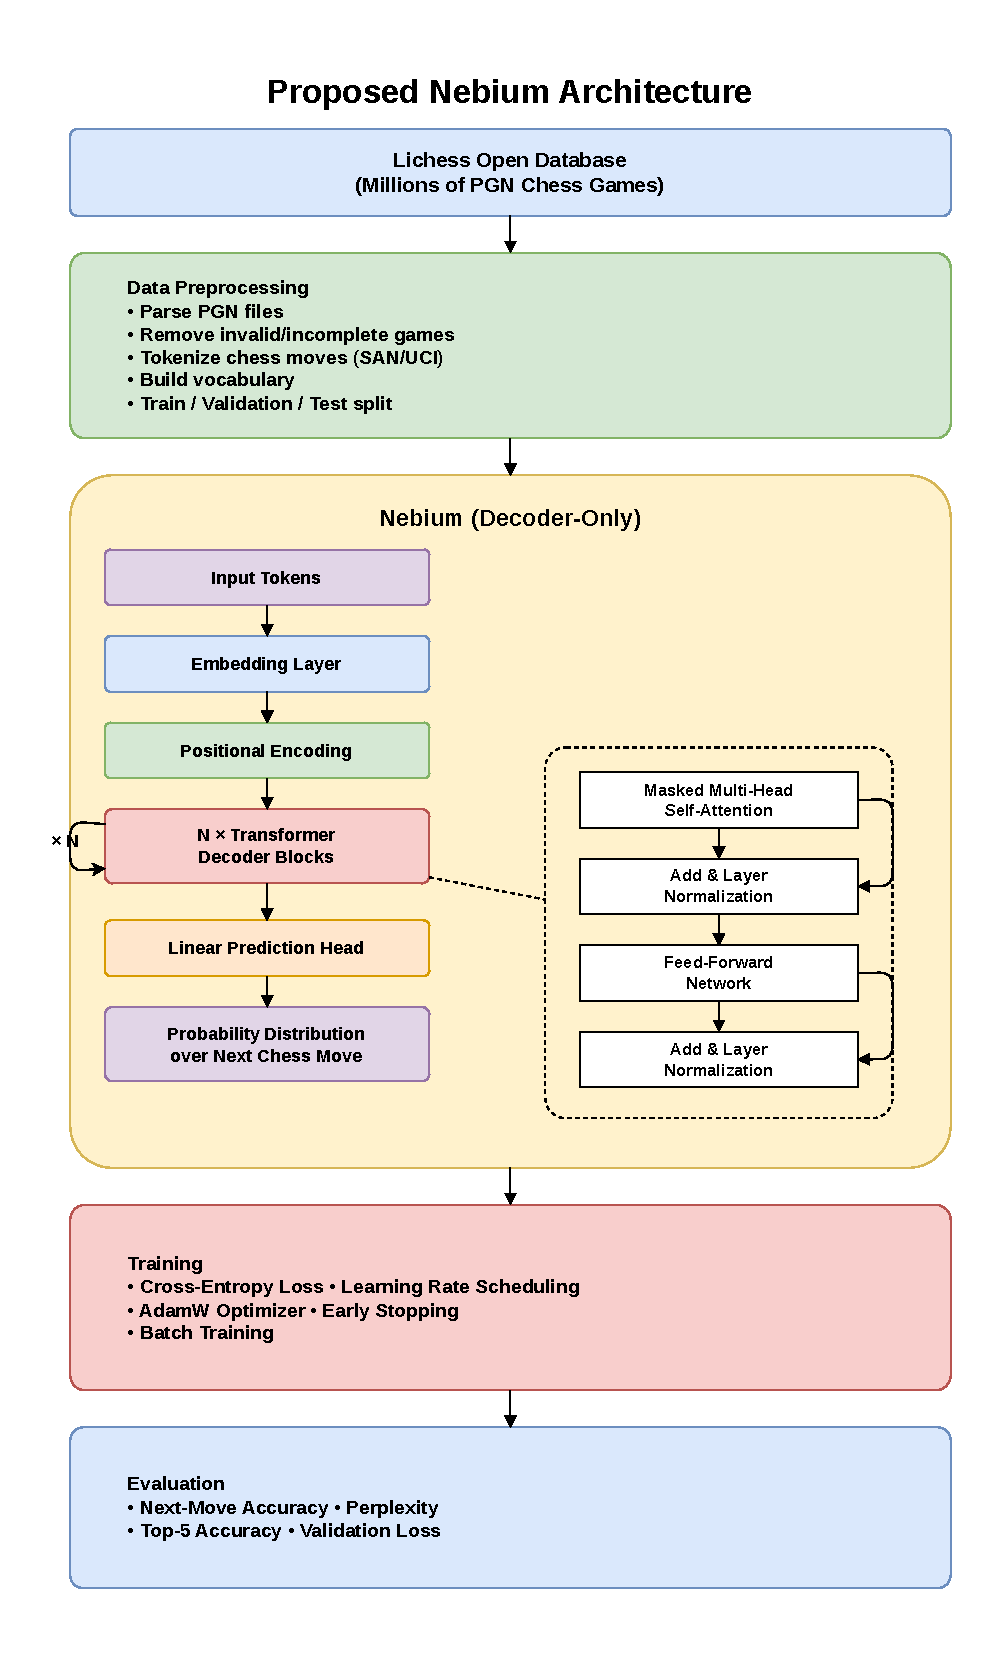
\includegraphics[width=0.78\linewidth]{figures/nebium.pdf}
  \caption[Nebium Causal Transformer Architecture]{Architectural overview of the Nebium causal transformer. Tokenized UCI move prefixes pass through token embedding, rotary position encoding, stacked pre-normalized causal transformer blocks, and a linear language modeling head.}
  \label{fig:architecture}
\end{figure}

\subsection{Rotary Position Embeddings (RoPE)}
\label{sec:rope_method}
Traditional language models rely on absolute learned position embeddings $\mathbf{p}_t \in \mathbb{R}^{d_{\text{model}}}$ added directly to the token embedding ($\mathbf{e}_t + \mathbf{p}_t$). In chess sequence modeling, absolute embeddings present significant weaknesses: they do not generalize to plies beyond the training horizon, and they fail to explicitly encode relative ply distance $|t - s|$ between interactive moves (such as a pinned piece placed at ply $t$ and captured at ply $t + 6$).

Nebium employs Rotary Position Embeddings (RoPE) \parencite{su2024roformer}, which encode positional context by directly rotating query and key representations in the complex plane. Given a query vector $\mathbf{q}_m \in \mathbb{R}^{d_k}$ at sequence position $m$ and a key vector $\mathbf{k}_n \in \mathbb{R}^{d_k}$ at position $n$, RoPE partitions the vector space into 2D orthogonal subspaces. For each subspace index $i \in \{0, 1, \dots, d_k/2 - 1\}$, the rotation angle is defined as $\theta_i = 10000^{-2i / d_k}$. The 2D rotation matrix is given by:
\begin{equation}
    \mathbf{R}_{\Theta, m}^{(i)} = 
    \begin{pmatrix}
        \cos(m \theta_i) & -\sin(m \theta_i) \\
        \sin(m \theta_i) & \cos(m \theta_i)
    \end{pmatrix}
\end{equation}
The inner product between the rotated query and key vectors naturally isolates the relative temporal distance $m - n$:
\begin{equation}
    \langle \mathbf{R}_{\Theta, m} \mathbf{q}_m, \, \mathbf{R}_{\Theta, n} \mathbf{k}_n \rangle = \mathbf{q}_m^T \mathbf{R}_{\Theta, n - m} \mathbf{k}_n = g(\mathbf{q}_m, \mathbf{k}_n, m - n)
\end{equation}
Consequently, self-attention scores between pieces naturally reflect relative move latencies and turn-taking tempos, allowing the model to extrapolate across extended endgames.

\subsection{Multi-Head Causal Self-Attention}
\label{sec:mhsa_method}
The attention mechanism in Nebium implements scaled dot-product causal attention across $h = 8$ parallel heads. Query, Key, and Value projections are computed as linear transformations without bias:
\begin{equation}
    \mathbf{Q} = \mathbf{X} \mathbf{W}_Q, \quad \mathbf{K} = \mathbf{X} \mathbf{W}_K, \quad \mathbf{V} = \mathbf{X} \mathbf{W}_V, \quad \mathbf{W}_Q, \mathbf{W}_K, \mathbf{W}_V \in \mathbb{R}^{d_{\text{model}} \times d_{\text{model}}}
\end{equation}
After rotary transformation is applied to $\mathbf{Q}$ and $\mathbf{K}$, the causal attention matrix is computed. To preserve temporal autoregression, an upper-triangular causal attention mask $\mathbf{M} \in \{0, -\infty\}^{T \times T}$ is applied:
\begin{equation}
    \mathbf{M}_{i, j} = 
    \begin{cases}
        0, & \text{if } i \ge j \\
        -\infty, & \text{if } i < j
    \end{cases}
\end{equation}
The attention weights and aggregated output are calculated via:
\begin{equation}
    \text{Attention}(\mathbf{Q}, \mathbf{K}, \mathbf{V}) = \text{softmax}\left( \frac{\mathbf{Q} \mathbf{K}^T}{\sqrt{d_k}} + \mathbf{M} \right) \mathbf{V}
\end{equation}
Nebium dynamically invokes PyTorch's native Scaled Dot-Product Attention (\texttt{scaled\_}\allowbreak\texttt{dot\_}\allowbreak\texttt{product\_}\allowbreak\texttt{attention}), unlocking hardware-accelerated FlashAttention kernels that eliminate memory bandwidth bottlenecks during backpropagation.

\subsection{SwiGLU Feed-Forward Network}
\label{sec:swiglu_method}
Standard transformers use a two-layer feed-forward network with Gaussian Error Linear Units (GELU) \parencite{vaswani2017attention}. Nebium instead replaces this block with the Swish-Gated Linear Unit (SwiGLU) \parencite{shazeer2020glu}, which applies multiplicative gating over intermediate representations. For an input vector $\mathbf{x} \in \mathbb{R}^{d_{\text{model}}}$:
\begin{equation}
    \text{SwiGLU}(\mathbf{x}) = \left( \text{SiLU}\left(\mathbf{x} \mathbf{W}_{\text{gate}}\right) \odot \left(\mathbf{x} \mathbf{W}_{\text{up}}\right) \right) \mathbf{W}_{\text{down}}
\end{equation}
where $\text{SiLU}(z) = z \cdot \sigma(z) = \frac{z}{1 + e^{-z}}$, $\odot$ denotes element-wise multiplication, and projection matrices are defined as $\mathbf{W}_{\text{gate}}, \mathbf{W}_{\text{up}} \in \mathbb{R}^{d_{\text{model}} \times d_{ff}}$ and $\mathbf{W}_{\text{down}} \in \mathbb{R}^{d_{ff} \times d_{\text{model}}}$.

Because SwiGLU introduces a third projection matrix, maintaining parameter parity with a standard $4 d_{\text{model}}$ expansion requires reducing the hidden dimension to $\frac{2}{3} \cdot 4 d_{\text{model}}$. To align with GPU tensor core memory tiles, $d_{ff}$ is rounded to the nearest multiple of 8:
\begin{equation}
    d_{ff} = 8 \times \left\lfloor \frac{\frac{2}{3} \times 4 \times d_{\text{model}} + 7}{8} \right\rfloor = 1,368
\end{equation}
This preserves parameter equivalence with a conventional 2-layer FFN while enabling gated non-linear transformations.

\subsection{Root Mean Square Layer Normalization (RMSNorm)}
\label{sec:rmsnorm_method}
Standard Layer Normalization enforces zero-mean and unit-variance across feature dimensions:
\begin{equation}
    \text{LayerNorm}(\mathbf{x}) = \frac{\mathbf{x} - \mu}{\sqrt{\sigma^2 + \epsilon}} \odot \boldsymbol{\gamma} + \boldsymbol{\beta}, \quad \mu = \frac{1}{d}\sum_{i=1}^d x_i, \quad \sigma^2 = \frac{1}{d}\sum_{i=1}^d (x_i - \mu)^2
\end{equation}
\textcite{zhang2019root} demonstrated that the stabilization benefit of LayerNorm derives primarily from scaling by the root mean square, rendering the mean-centering step computationally dispensable. Nebium adopts RMSNorm, normalizing inputs strictly by their root mean square:
\begin{equation}
    \text{RMSNorm}(\mathbf{x}) = \frac{\mathbf{x}}{\text{RMS}(\mathbf{x})} \odot \boldsymbol{\gamma}, \quad \text{where } \text{RMS}(\mathbf{x}) = \sqrt{\frac{1}{d}\sum_{i=1}^d x_i^2 + \epsilon}
\end{equation}
where $\boldsymbol{\gamma} \in \mathbb{R}^{d_{\text{model}}}$ is a learnable gain parameter and $\epsilon = 10^{-6}$ prevents division by zero. Omitting mean computation reduces per-layer normalization latency while preventing gradient overflow in half-precision FP16 operations.

\subsection{Inference Engine and Dynamic Legal Move Masking}
\label{sec:legal_masking}
During inference, the model processes a sequence of historical move tokens $\mathbf{x}_{<t}$ and outputs unnormalized logits $\mathbf{z}_t \in \mathbb{R}^V$ over the move vocabulary. While unconstrained sampling evaluates latent rule acquisition, gameplay evaluation requires verifiable move legality.

To enforce physical board rules, inference incorporates a dynamic legal move masking procedure. At ply $t$, the board state $s_t$ is synchronized using \texttt{python-chess} \parencite{romstad2024pythonchess}. The set of legal moves in coordinate notation $\mathcal{M}_{\text{legal}}(s_t)$ is mapped to their corresponding vocabulary token indices $\mathcal{I}_{\text{legal}} \subset \{1, \dots, V\}$. Non-legal logits are set to negative infinity:
\begin{equation}
    \tilde{z}_{t, i} = 
    \begin{cases}
        z_{t, i} / \tau, & \text{if } i \in \mathcal{I}_{\text{legal}} \\
        -\infty, & \text{otherwise}
    \end{cases}
\end{equation}
where $\tau > 0$ controls sampling temperature. The final move probability is computed over the restricted support:
\begin{equation}
    P(x_t = i \mid \mathbf{x}_{<t}) = \frac{\exp(\tilde{z}_{t, i})}{\sum_{j \in \mathcal{I}_{\text{legal}}} \exp(\tilde{z}_{t, j})}
\end{equation}
This mechanism restricts generation strictly to valid moves while preserving the model's relative probability ranking over legal candidates.

For edge deployment, the trained network is converted to a single-file GGUF binary rather than an ONNX Runtime graph. As outlined in Section~\ref{sec:tools_deployment}, ONNX exports separate computation graphs from tokenization code and incur Python runtime overhead on sequential token queries. GGUF embeds weights, 4-bit block quantization scales (\texttt{Q4\_K\_M}), and vocabulary metadata in a single file, supporting memory-mapped C++ execution on consumer CPUs without external runtime dependencies.
